% Elsevier elsarticle numeric submission template for JISA; see venue_template_jisa/COMPLIANCE.md.
% The review option increases line spacing for peer review; final production layout is set by Elsevier.
\documentclass[preprint,review,12pt]{elsarticle}
\usepackage{amsmath,amssymb,amsthm,booktabs,graphicx,tabularx}
\usepackage{lineno}
\usepackage[hidelinks]{hyperref}
\pdfstringdefDisableCommands{\def\corref#1{}}
\newtheorem{proposition}{Proposition}
\newtheorem{lemma}{Lemma}
\newcommand{\F}{\mathcal{F}_k}
\newcommand{\ind}{\mathbf{1}}
\journal{Journal of Information Security and Applications}
\begin{document}
\begin{frontmatter}
\title{Zero-Knowledge Certification of Robust Spacetime Compliance under Byzantine Evidence for Vehicular Crowdsensing}
% Author order, affiliation and correspondence supplied by the user on 2026-09-22.
\author[aff1]{Lili He}
\author[aff1]{Sheng Jiang}
\author[aff1]{Linghui Lyu}
\author[aff1]{Lei Zhang\corref{cor1}}
\cortext[cor1]{Corresponding author: Lei Zhang.}
\ead{8213662@163.com}
\affiliation[aff1]{organization={College of Information and Electronic Technology, Jiamusi University},
city={Jiamusi},postcode={154007},country={China}}
\begin{abstract}
Privacy-preserving location proofs typically certify a predicate over one hidden coordinate, but cryptographic correctness does not guarantee that the underlying event is well supported when positioning is uncertain or authenticated sources can be Byzantine. We address this gap by defining a report-bound security relation over private signed spacetime uncertainty boxes. Given explicit Byzantine and honest-miscoverage budgets, a report is accepted only when every threshold-supported state lies inside the authorized policy; ambiguous and inconsistent evidence are represented explicitly rather than coerced into a binary outcome. We realize the relation with two exact Groth16/BN254 circuits that verify EdDSA/MiMC-signed evidence and bind proofs to the task, roster, report, threshold, challenge, and expiry. Adversarial gateway tests reject evidence tampering, decision and report substitution, expired or unknown challenges, and cross-challenge replay; an eight-copy concurrent replay accepts exactly one copy. Across 12 predefined calibrated synthetic conditions, the robust rule provides 87.52\% mean decisive coverage versus 75.63\% for a fixed-margin rule. In the tested focus conditions, no wrong decisive output is observed whenever the theorem premise $M\le r$ holds. A same-stack hidden-point circuit requires 408--612 constraints, whereas the smallest authenticated robust circuits require 32,474--35,248 constraints, quantifying the cost of the stronger relation. Subset circuits produce 164-byte proofs with 163--255~ms median proving time on an Apple M1. These results validate the security relation and implementation, not field calibration: physical acceptance remains conditional on trusted enrollment and calibrated source coverage.
\end{abstract}
\begin{keyword}
Zero-knowledge proofs \sep Privacy-preserving verification \sep Byzantine evidence \sep Robust sensor fusion \sep Location privacy \sep Vehicular crowdsensing
\end{keyword}
\end{frontmatter}
\linenumbers
\section{Introduction}
Privacy-preserving verification is often framed as proving that one hidden attribute satisfies a public predicate. For location-sensitive services, this can mean proving that a hidden coordinate lies in an authorized region without revealing the coordinate~\cite{ZKLP,VehiclePolicy}. The cryptographic statement can nevertheless be correct while the underlying physical claim is weakly supported: location and time estimates are uncertain, an authenticated source can be miscalibrated, and a compromised source can sign deliberately misleading evidence. The security question is therefore not only whether one hidden point satisfies a policy, but whether the available authenticated uncertainty evidence supports that policy robustly.

Vehicular crowdsensing provides a concrete instance of this problem. Mobile crowdsensing pools observations from participating devices~\cite{Suhag2023}, while vehicle-based systems use distributed sensing for transportation and environmental tasks~\cite{Zheng2025BARM}. A report may be eligible only when its reference event occurs in a specified region and time window, yet disclosing raw positioning evidence or a precise trajectory can expose sensitive mobility information. Near a policy boundary, selecting one convenient point from an uncertainty range can make an existential location proof succeed even when other plausible states violate the policy. Intersecting all source ranges is also unsafe under Byzantine evidence because a compromised source can exclude the true state while retaining a small compliant intersection.

We formulate the problem as a privacy-preserving security relation over authenticated uncertainty. Each enrolled issuer signs an axis-aligned integer box for the same report-bound reference event. With $n$ issuers, Byzantine budget $f$, honest-miscoverage budget $r$, and threshold $k=n-f-r$, the robust feasible set contains every state supported by at least $k$ signed boxes. A report is authorized only when this set is nonempty and entirely contained in the public policy. Separate reachability predicates inside and outside the policy distinguish valid, invalid, ambiguous, and inconsistent evidence instead of forcing every event into a binary decision.

The construction combines established fault-tolerant fusion ideas~\cite{Marzullo1990,BFTPoLoc,PG,CRSF} with zero-knowledge certification. The novelty is not a new SNARK primitive or a new sensor-fusion theorem. It is the security composition that turns robust uncertain evidence into a private, report-bound compliance certificate and makes the trust and calibration assumptions explicit.

The main contributions are:
\begin{itemize}
 \item We define robust spacetime-compliance semantics for signed uncertainty boxes under explicit Byzantine and honest-miscoverage budgets. The four-valued decision prevents vacuous acceptance and yields a conditional soundness statement that separates cryptographic validity from physical coverage assumptions.
 \item We give two exact finite-domain realizations of the relation: lower-corner maximum-depth reachability and threshold-subset enumeration. Both circuits verify issuer signatures in Groth16 and bind the private boxes to the public policy, roster, threshold, report context, challenge, and expiry.
 \item We implement a task-authorized gateway that reconstructs trusted public inputs, rejects roster/key inconsistencies, verifies the proof, and atomically consumes a challenge after successful verification. The resulting protocol addresses witness tampering, cross-task/report substitution, and same-challenge replay within the stated local model.
 \item We evaluate semantics and implementation separately. The study includes 64,800 synthetic observations, matched analyses across miscoverage budgets, a 787-state UrbanNav reference-trajectory replay with simulated evidence, 300 measured Groth16 proofs across two backends, a resource-bounded compilation sweep, and a pinned same-runner reproduction of the closest open-source ZK location baseline. These experiments validate the implemented security relation and its cost; they are not presented as field calibration of real multisource vehicular positioning.
\end{itemize}

Figure~\ref{fig:architecture} summarizes the evidence-to-proof boundary. The verifier learns the public task inputs and the classification, while the signed uncertainty boxes and their signatures remain private witnesses.
\begin{figure}[htbp]
\centering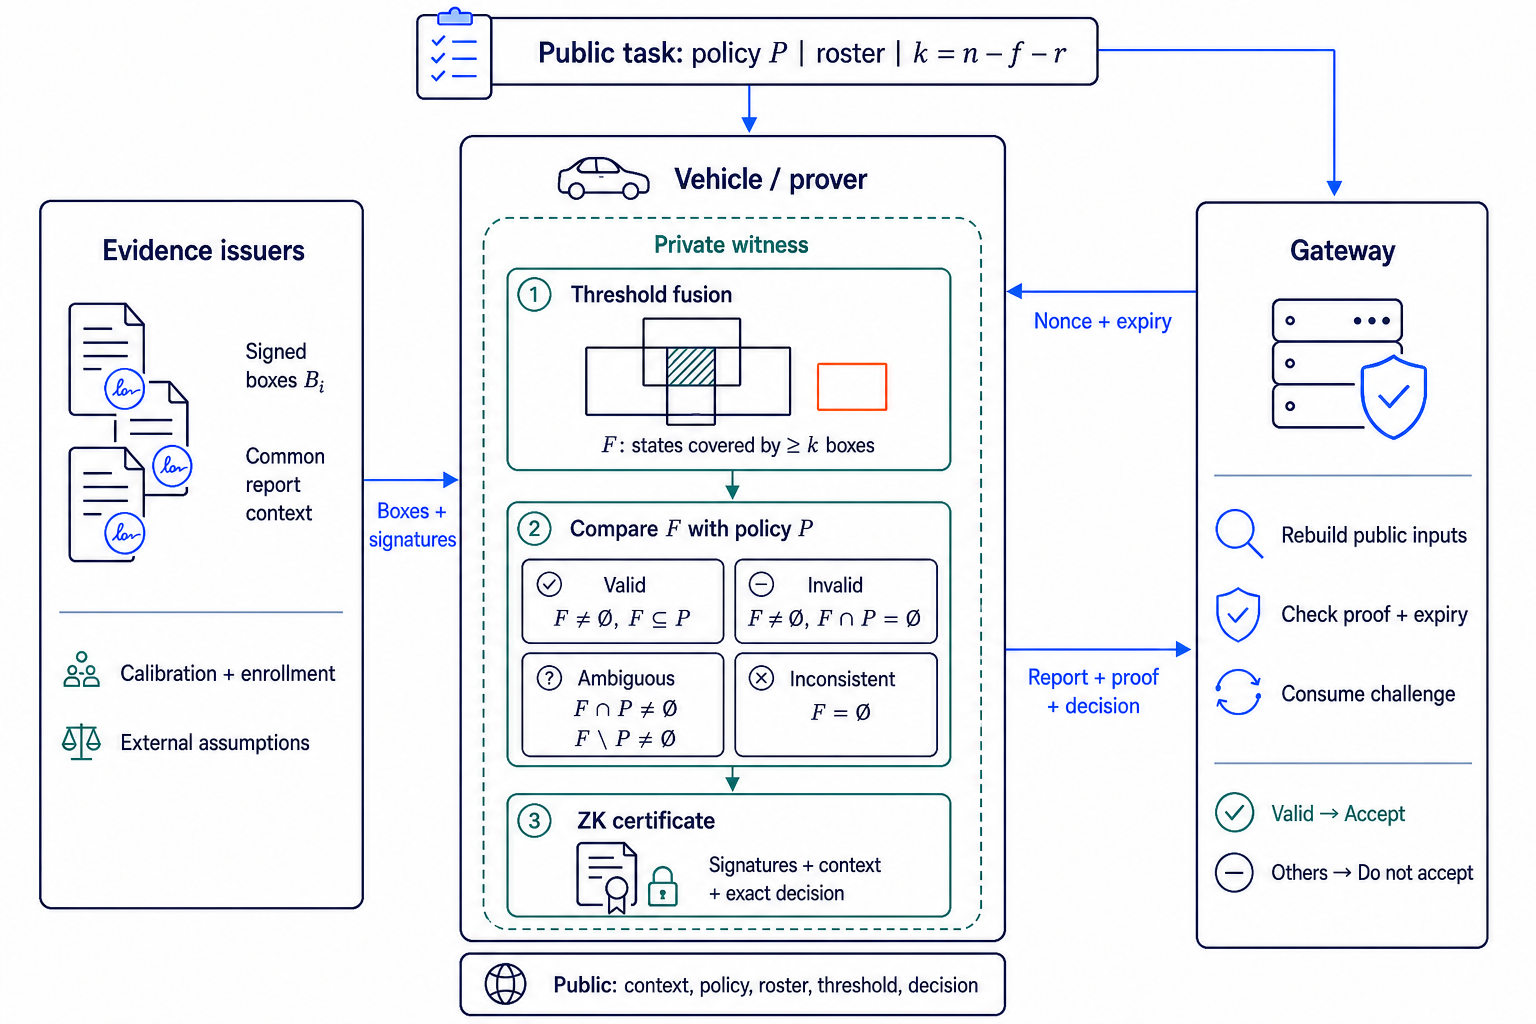
\includegraphics[width=\linewidth]{figures/system_architecture.png}
\caption{Conceptual architecture of the local prototype. The diagram's $B_i$ and $F$ denote the evidence boxes $U_i$ and feasible set $\F$ used in the text. Issuers sign boxes bound to a common report context; the vehicle proves the robust decision using private evidence. The gateway checks the task-bound proof and expiry, consumes a verified challenge, and accepts only a valid decision. ``Inconsistent'' means proved evidence failure, not a missing signature. Calibration and trusted enrollment remain external assumptions. Icons do not imply physical issuer independence or deployment. Initial schematic generated using OpenAI image generation through Codex (model version not exposed in the retained workflow) and reviewed by the authors for technical accuracy.}\label{fig:architecture}
\end{figure}

Subset enumeration is the practical choice in the measured small-omission regime. The depth construction instead permits a public threshold and has a polynomial bound at fixed dimension; the matched experiments compare their costs without claiming a universal crossover.
\section{Related work and security positioning}
Vehicular privacy work spans authentication, protected aggregation, location privacy, and misbehavior detection. AARE and BARM combine anonymous participation with reliability or reputation mechanisms~\cite{Cheng2023,Zheng2025BARM}; PPVDA protects and verifies sensing aggregation~\cite{Zhou2024}; BCS-LPP protects sensing locations~\cite{Shen2024}; and cooperative Sybil detection fuses motion and roadside evidence~\cite{Sultana2024}. Recent JISA studies similarly emphasize anonymous authentication, aggregate signatures, and authenticated-data SNARKs~\cite{Imam2025JISA,Wang2025JISA,Reinhart2026ADSC}. These systems secure identities, inputs, or computations, whereas our certified object is whether private uncertain evidence robustly supports a public spacetime policy.

Location-privacy mechanisms range from application-aware obfuscation~\cite{Mdee2022,Atmaca2024} to authentication and Sybil-resistant credentialing~\cite{Ghani2025,Zhang2025Sybil,Wang2025ZKAuth}. The closest zero-knowledge formulations are ZKLP's private geometric predicates~\cite{ZKLP} and signed-trajectory policy proofs for vehicle subsidies and taxation~\cite{VehiclePolicy}. They motivate private policy verification but do not model threshold-supported uncertainty under Byzantine evidence.

Robust fusion originates in fault-tolerant interval reasoning~\cite{Marzullo1990}. BFT-PoLoc applies Byzantine-resistant geometry to Internet-delay location inference~\cite{BFTPoLoc}, while PG and CRSF protect Byzantine sensor fusion and participation in distributed secure-computation settings~\cite{PG,CRSF}. Our fixed-roster prototype does not inherit their liveness guarantees; it produces a portable proof of a four-valued policy decision over signed uncertainty boxes. Table~\ref{tab:related-work} summarizes these different certification targets.
\begin{table}[htbp]
\centering
\renewcommand{\baselinestretch}{1}\footnotesize
\setlength{\tabcolsep}{4pt}
\renewcommand{\arraystretch}{1.08}
\caption{Functional comparison of related systems. Each row uses its own evidence and trust assumptions; this is not a performance ranking.}
\label{tab:related-work}
\begin{tabularx}{\linewidth}{@{}>{\hsize=.65\hsize\raggedright\arraybackslash}X>{\hsize=.95\hsize\raggedright\arraybackslash}X>{\hsize=1.15\hsize\raggedright\arraybackslash}X>{\hsize=1.25\hsize\raggedright\arraybackslash}X@{}}
\toprule
Work&Checked object&Evidence / trust model&Privacy / output interface\\
\midrule
\multicolumn{4}{@{}l}{\textit{Vehicular crowdsensing and participation}}\\[1pt]
BARM~\cite{Zheng2025BARM}\newline(2025)&Identity and reputation&Reputation evaluation; blockchain identity management&Anonymous authentication; private reputation evaluation and updates\\[2pt]
PPVDA~\cite{Zhou2024}\newline(2024)&Inner-product aggregate&Homomorphic MACs; secret sharing; malicious model&Private sensing inputs; verifiable aggregate\\[2pt]
BCS-LPP~\cite{Shen2024}\newline(2024)&Sensing locations&Geohash; order-preserving encryption; deposits&Location privacy levels; location validation and task management\\
\midrule
\multicolumn{4}{@{}l}{\textit{Robust inference and private sensor fusion}}\\[1pt]
BFT-PoLoc~\cite{BFTPoLoc}\newline(2024)$^{\dagger}$&IP-address location&Internet delays; Byzantine-resistant geometry&Distance estimates and multilateration; privacy not assessed here\\[2pt]
PG~\cite{PG}\newline(2024)&Sensor fusion&Malicious sensors and aggregation servers&Private inputs and fusion result; guaranteed output delivery\\[2pt]
CRSF~\cite{CRSF}\newline(2026)$^{\dagger}$&Fusion and participation&Sensor--server collusion; agreement on submissions&Private fusion; explicit abort and liveness guarantees\\
\midrule
\multicolumn{4}{@{}l}{\textit{Zero-knowledge geometry and policy certification}}\\[1pt]
ZKLP~\cite{ZKLP}\newline(2025)&Region membership; proximity&Private coordinates; floating-point geometry&Hidden coordinates; zero-knowledge geometric proofs\\[2pt]
Vehicle policy~\cite{VehiclePolicy}\newline(2025)&Territorial driving requirements&Location claims signed by a trusted witness&Hidden trajectory; subsidy / taxation compliance proofs\\[2pt]
\textbf{This work}&\textbf{All threshold-supported event states}&Signed boxes; fixed roster; Byzantine budget $f$ and honest-miss budget $r$&Private boxes and signatures; portable proof of a four-valued policy decision\\
\bottomrule
\end{tabularx}
\par\vspace{4pt}\raggedright
$^{\dagger}$Cited as preprints. MAC: message authentication code. Privacy guarantees depend on each protocol's public outputs. Our four decisions are valid, invalid, ambiguous, and inconsistent; missing signatures instead cause protocol abort.
\end{table}

Generic secure computation could evaluate the same finite decision function. Our contribution is the signed-box relation, report binding, exact circuit realizations, and measured security/performance tradeoffs; no new cryptographic primitive is claimed.
\section{Evidence and adversary model}
The reference event is $z^\star=(x,y,t)$, or generally a point in
\begin{equation}
 \Omega=\prod_{a=1}^{d}[L_a,H_a]\cap\mathbb{Z}^d.
\end{equation}
A public policy is an integer box $P\subseteq\Omega$, and issuer $i$ signs an inclusive integer uncertainty box $U_i\subseteq\Omega$ under a common context $c$. Coordinates share a public frame, epoch, units, and quantization rule; the prototype uses unsigned 16-bit bounds. Exactness therefore refers to this finite model, not to unquantized physical space.

Signatures authenticate submitted bounds but not their physical accuracy. We assume at most $f$ Byzantine issuers and at most $r$ additional honest boxes that miss $z^\star$; honest errors may be dependent. The counted unit is an enrolled authority, not merely a public key, so multiple keys or estimates under common control do not create independent trust domains~\cite{Zhang2025Sybil}. A missing roster signature aborts the protocol rather than producing an ``inconsistent'' decision.

\paragraph{Trust boundary.}
The vehicle and network are untrusted and may alter, replay, reorder, or substitute reports, proofs, decisions, and challenges. Byzantine issuers may choose arbitrary policy-aware boxes under their own keys. Honest issuers protect signing keys and bind evidence to the intended context, while the gateway's task configuration, verifying key, clock, and roster are trusted. The adversary is computationally bounded and is not assumed to break the underlying proof, signature, or hash primitives. Witness confidentiality is claimed against the verifier, not against evidence issuers or an administrator allowed unrestricted adaptive policy queries.

The public statement contains $c$, $\Omega$, $P$, threshold $k$, a decision code, and ordered issuer keys. Issuer $i$ signs
\begin{equation}
 m_i=\operatorname{MiMC}(c,i,\ell_{i1},u_{i1},\ldots,\ell_{id},u_{id}).
\end{equation}
The context binds protocol/task identifiers, coordinate convention, calibration profile, domain, policy, threshold, roster, report digest, challenge nonce, and expiry. The gateway reconstructs these values from its trusted task snapshot instead of accepting a vehicle-selected public witness.

\paragraph{Physical and liveness scope.}
A deployable issuer must conservatively map a common physical event into the configured frame and uncertainty box using validated calibration. Radio ranging, roadside perception, synchronization, non-line-of-sight bias, frame registration, and common-mode failures are outside the prototype. Likewise, one withholding roster member can abort the fixed-roster protocol. Supporting partial participation would require an authenticated active set with its own fault/coverage budget; simply dropping missing issuers while retaining the old threshold is unsound. The current design therefore targets provisioned, delay-tolerant checks rather than opportunistic safety-critical V2X control.

For continuous coordinates, evidence should conservatively include every quantized cell intersecting the physical uncertainty region, while acceptance should require cells wholly inside the policy. The implemented single-policy integer relation does not supply this continuous-to-discrete adapter; out-of-range values must be rejected rather than clamped.
\subsection{Report binding and challenge lifecycle}
An administrator configures a task and its verifying key. The gateway snapshots the task configuration and rejects duplicated issuer keys or trust-domain labels. Labels enforce the administrator's enrollment decision; they do not prove independence of the underlying authorities. It issues a random 256-bit nonce with an expiry, using a trusted application clock. The vehicle and issuers derive
\begin{equation}
 c=\operatorname{OS2IP}\left(\operatorname{SHA256}(\operatorname{Encode}(v,T,\nu,e,\operatorname{SHA256}(R)))\right)\bmod q,
\end{equation}
\begin{sloppypar}
where $T$ is the configured task, $R$ the report bytes, $\nu$ the nonce, $e$ the expiry, and $q$ the BN254 scalar-field modulus. The prototype serializes a fixed-order, map-free Go JSON structure containing version, task, challenge, and the lowercase hexadecimal SHA-256 report digest; issuer key byte arrays use Go's base64 JSON encoding. This deterministic prototype encoding is language-bound, so cross-language deployments should reproduce the exact bytes or replace it with a separately specified canonical encoding. SHA-256 reduction binds context; it is not encryption.
\end{sloppypar}

At submission the gateway checks the nonce and expiry, reconstructs the trusted public witness, verifies the proof, and accepts only the valid class. Successful verification atomically consumes the nonce; an eight-way replay test therefore admits one copy. Failed proofs leave the challenge reusable until expiry, enabling benign retries but also invalid-proof CPU exhaustion, so deployment requires rate limiting. Fresh challenges can still carry duplicate reports, and restart persistence or distributed atomicity is not implemented.

Figure~\ref{fig:sequence} separates challenge issuance, evidence signing, and submission-time verification.
\begin{figure}[htbp]
\centering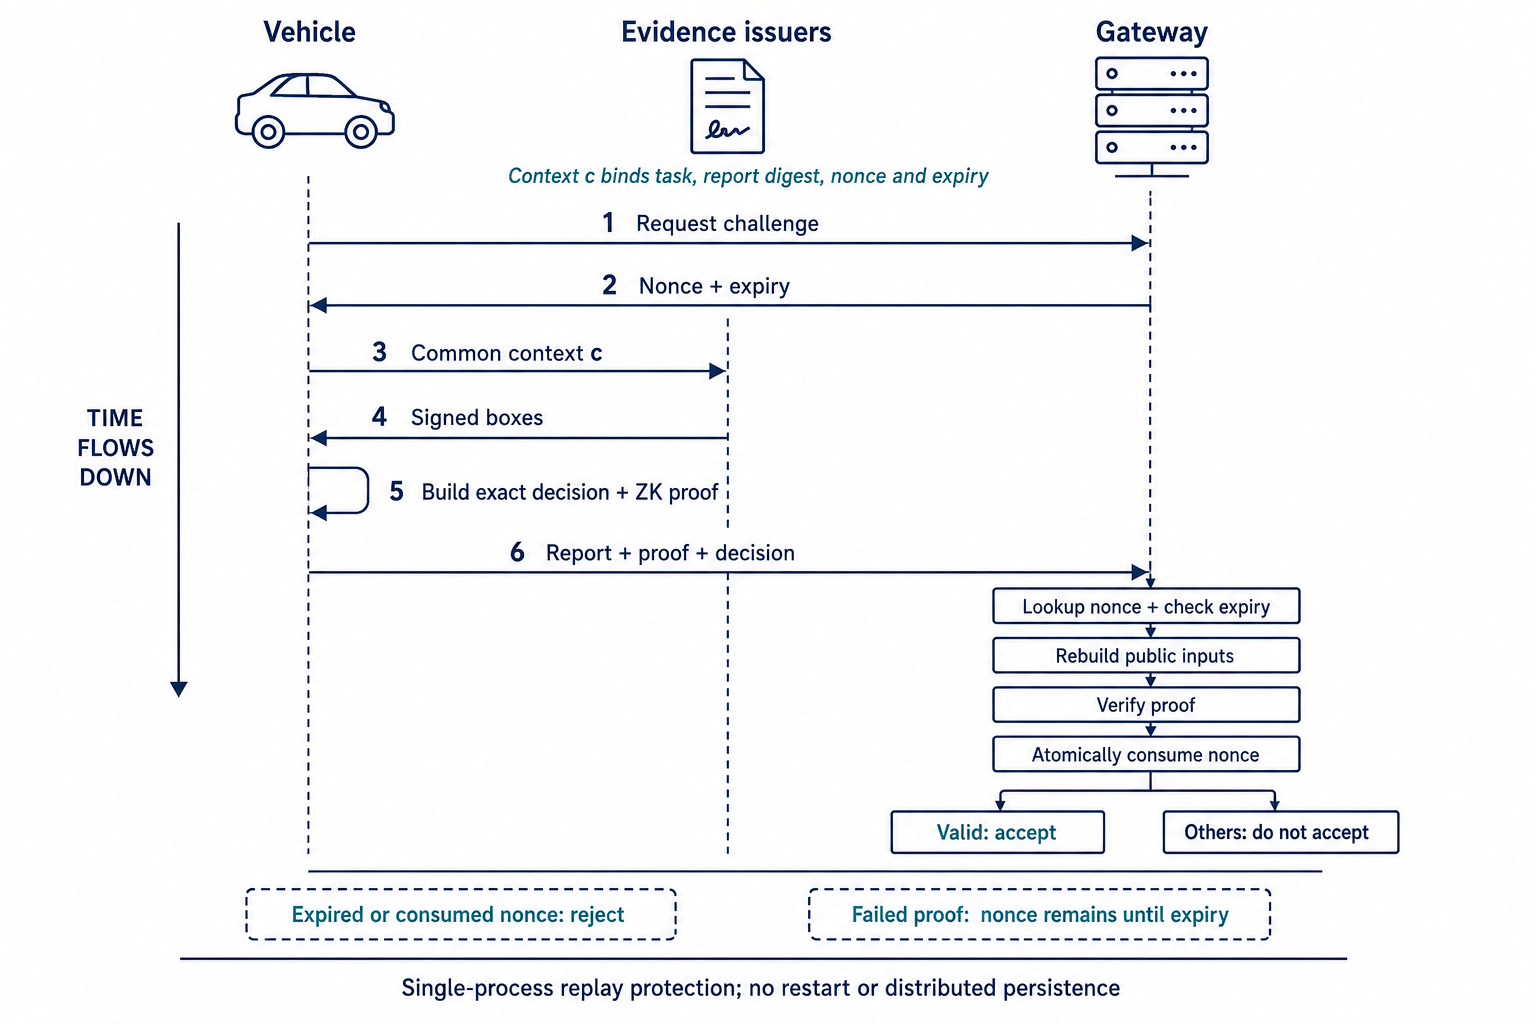
\includegraphics[width=\linewidth]{figures/protocol_sequence.png}
\caption{Report-bound challenge lifecycle. Successful verification consumes the nonce atomically; failed proofs do not. Transport is abstracted. Initial schematic generated using OpenAI image generation through Codex (model version not exposed in the retained workflow) and reviewed by the authors for technical accuracy.}\label{fig:sequence}
\end{figure}

\subsection{Security objectives and non-goals}
The evaluated properties are evidence authenticity, context integrity, conditional acceptance soundness, witness confidentiality, freshness, and fail-closed handling. Table~\ref{tab:security-properties} states their assumptions and validation evidence.

The design does not provide source availability, physical calibration, anonymous networking, Sybil-resistant enrollment, unlinkability, or privacy against unrestricted adaptive policy queries. Task policies are therefore assumed to be administrator-authorized and bound into the challenge context.

\begin{table}[htbp]
\centering\footnotesize
\caption{Security properties, dependencies, and validation evidence.}
\label{tab:security-properties}
\begin{tabularx}{\linewidth}{@{}>{\raggedright\arraybackslash}p{0.20\linewidth}>{\raggedright\arraybackslash}p{0.27\linewidth}>{\raggedright\arraybackslash}X@{}}
\toprule
Property & Required assumptions & Mechanism / evidence\\
\midrule
Evidence authenticity & Issuer signing keys uncompromised outside the $f$ Byzantine budget & In-circuit EdDSA verification; modified signed bounds rejected\\
Context integrity & Trusted gateway task configuration; collision resistance of transcript hashing & Binding covers task, report, roster, threshold, challenge, and expiry; substitution tests rejected\\
Conditional acceptance soundness & Proof-system soundness; at most $f$ Byzantine issuers; at most $r$ honest misses & Four-valued robust relation; Propositions~\ref{prop:soundness} and~\ref{prop:gateway}; direct $M\le r$ diagnostic\\
Witness confidentiality & Zero-knowledge of the instantiated proof system; public outputs accepted as leakage & Private boxes and signatures remain witness data; public leakage boundary stated explicitly\\
Freshness & Trusted clock and atomic gateway state within one instance & Expiry and consume-after-verify; eight-copy replay test accepts one copy\\
Fail-closed handling & Correct gateway execution and complete configured roster & Missing/malformed evidence, wrong decisions, unknown challenges, and duplicate roster entries abort\\
\bottomrule
\end{tabularx}
\end{table}
\section{Robust compliance semantics}
For $1\leq k=n-f-r\leq n$, define
\begin{equation}\label{eq:feasible}
 \F=\{z\in\Omega:\sum_{i=1}^{n}\ind[z\in U_i]\geq k\}.
\end{equation}
Let $I=\ind[\F\cap P\neq\varnothing]$ and $O=\ind[\F\cap(\Omega\setminus P)\neq\varnothing]$. These two bits give all four outcomes in Table~\ref{tab:decisions}. The inconsistent outcome is called evidence failure in the implementation and result tables. Distinguishing it avoids vacuous acceptance: the empty set is mathematically a subset of every policy, but it supplies no evidence of a compliant event.

\begin{table}[htbp]
\centering
\caption{Exact decision semantics. Only valid authorizes acceptance.}\label{tab:decisions}
\begin{tabular}{cccl}
\toprule $I$ & $O$ & Code & Decision \\\midrule
1&0&0&Valid: nonempty feasible set contained in $P$\\
0&1&1&Invalid: nonempty feasible set disjoint from $P$\\
1&1&2&Ambiguous: feasible states on both sides\\
0&0&3&Inconsistent: no threshold-supported state\\\bottomrule
\end{tabular}
\end{table}

In the constructed example of Figure~\ref{fig:counterexample}, $\Omega=[-4,8]\cap\mathbb Z$ and both honest intervals contain $z^\star=-1$. The Byzantine interval excludes it. The all-source intersection $[2,4]\cap\mathbb Z$ lies inside the policy even though it excludes the true state, and a conveniently chosen point also passes. Threshold coverage retains $\F=[-2,4]\cap\mathbb Z$, giving an ambiguous decision. The example applies the existing fusion rationale; it supplies neither a new theorem nor an experimental success rate.
\begin{figure}[htbp]
\centering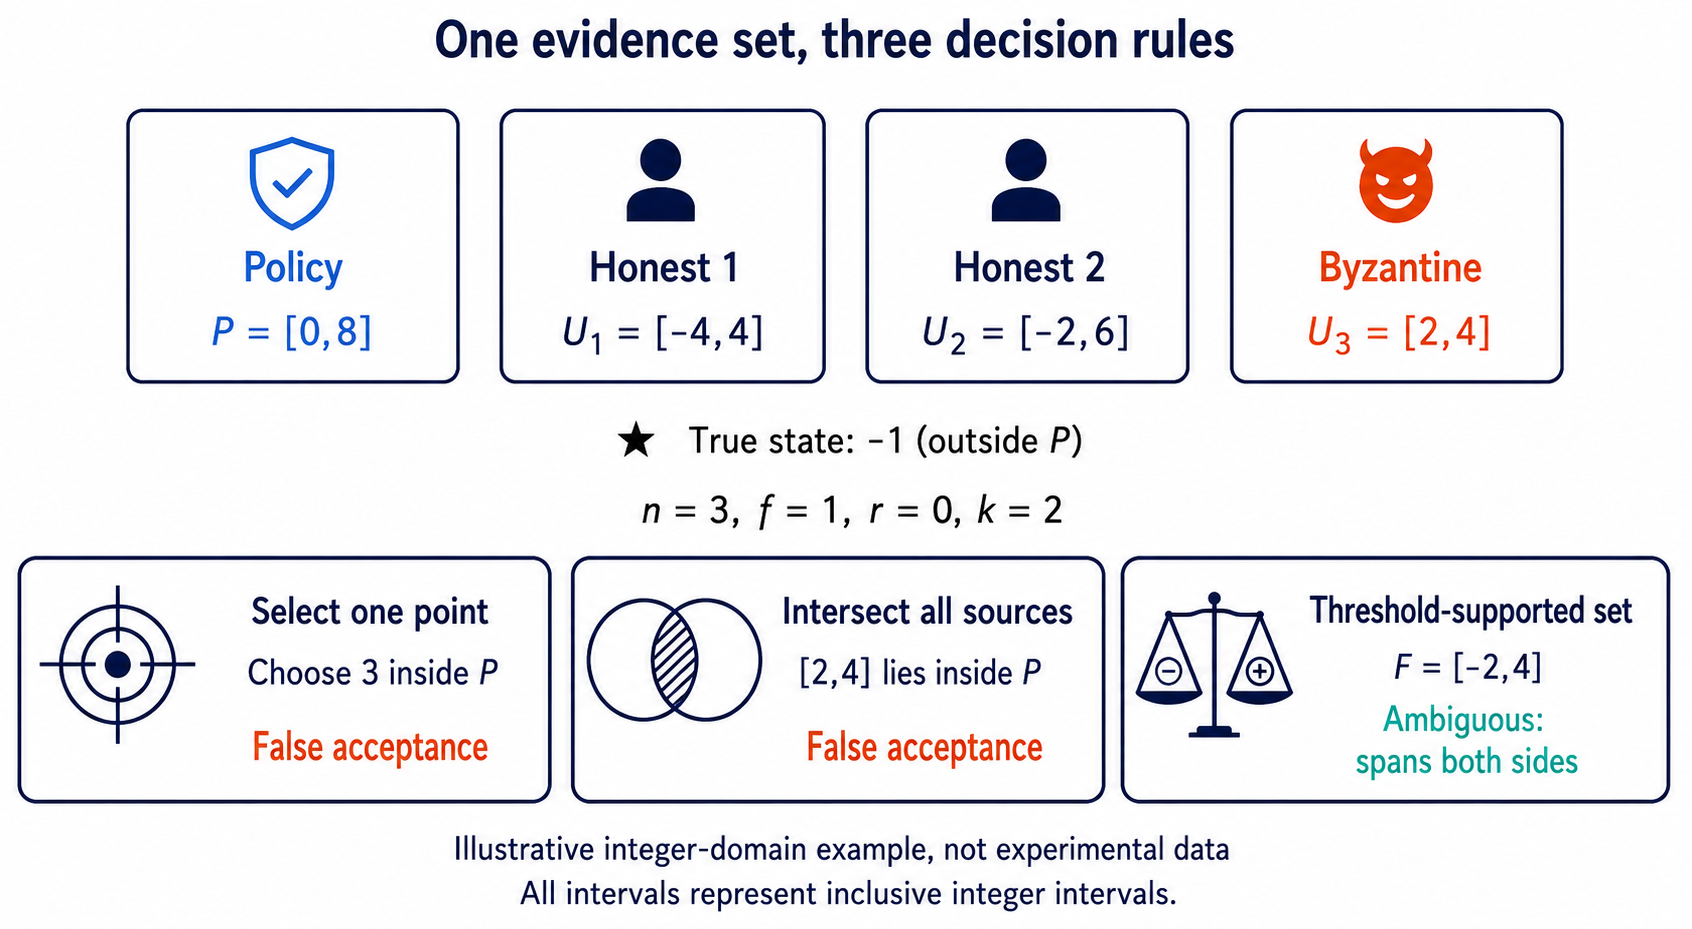
\includegraphics[width=\linewidth]{figures/decision_counterexample.png}
\caption{One evidence set under three rules. All intervals are inclusive integer sets; $n=3,f=1,r=0,k=2$. The two naive acceptance examples contradict the known noncompliant true state, whereas the robust set spans the policy boundary. This is a constructed explanatory example, not measured data. Initial schematic generated using OpenAI image generation through Codex (model version not exposed in the retained workflow) and reviewed by the authors for technical accuracy.}\label{fig:counterexample}
\end{figure}

\begin{proposition}[Conditional evidence soundness]\label{prop:soundness}
If at most $f$ issuers are Byzantine and at most $r$ honest boxes miss $z^\star$, then $z^\star\in\F$. Consequently, a valid decision implies $z^\star\in P$, and an invalid decision implies $z^\star\notin P$.
\end{proposition}
\begin{proof}
At least $n-f-r=k$ boxes contain the true state, so its coverage reaches the threshold in~\eqref{eq:feasible}. The two implications follow respectively from set containment and disjointness.\end{proof}
The proof uses the classical threshold-containment argument. The extra condition $n>2f+r$ guarantees at least one honest supporter for a threshold-supported point, but truth inclusion above does not require it.

For probabilistic calibration, let $M$ be the number of honest boxes missing the event and assume honest source $i$ has marginal failure probability at most $\alpha_i$ for the specified operating population. Without independence,
\begin{equation}\label{eq:calibration}
 \Pr(M>r)\leq \min\left(1,\frac{\sum_{i\in\mathcal H}\alpha_i}{r+1}\right).
\end{equation}
Indeed, $\mathbb{E}M\leq\sum_i\alpha_i$ and $M>r$ entails $M\geq r+1$. This loose bound does not supply missing calibration estimates. For adaptively chosen tasks, applicable conditional calibration or a suitable joint bound is required; a marginal guarantee from unrelated data is insufficient.

Under independent Bernoulli misses with known $\alpha_i$, a tighter Poisson-binomial tail is available, but shared positioning errors generally preclude using that bound. We therefore retain the dependence-agnostic guarantee in~\eqref{eq:calibration}.

\section{Finite proof construction}
\subsection{Lower-corner reachability}
For a query box $Q$, intersect each evidence box with $Q$. Let $A_a$ contain the lower endpoints of nonempty clipped boxes on axis $a$.
\begin{lemma}\label{lem:corner}
If the maximum overlap depth in $Q$ is positive, some maximizer belongs to $A_1\times\cdots\times A_d$.
\end{lemma}
\begin{proof}
Choose a maximum-depth point $z$ and all boxes covering it. Their intersections with $Q$ have a common intersection. Its lower corner $v$ is formed by taking the greatest lower endpoint on each axis, hence $v_a\in A_a$. Every selected box contains $v$, so its depth is at least that of $z$ and therefore maximal.\end{proof}
The circuit considers $n^d$ candidates, including duplicates, with coordinate $v_a=\max(\ell_{j_a a},Q^-_a)$. It tests query membership and coverage by every evidence box. Candidates associated with boxes not intersecting the query cannot cause false reachability because all membership comparisons are evaluated. Reachability is the OR of all candidate tests with depth at least $k$.

The integer complement $\Omega\setminus P$ is the union of at most $2d$ slabs. The low slab for axis $a$ ends at $p^-_a-1$ and the high slab begins at $p^+_a+1$. Other coordinates span the domain. Slabs can overlap. A slab beyond the domain boundary is inactive, with a safe selected endpoint before comparisons. The circuit computes $I$ over $P$ and $O$ over these slabs, then constrains the public code to
\begin{equation}
 \delta=(1-I)O+2IO+3(1-I)(1-O).
\end{equation}
All box coordinates are range-constrained, lower endpoints do not exceed upper endpoints, and boxes and policy lie within $\Omega$. Issuer signatures are checked inside the circuit. Pairwise public-key equality is forbidden.

\subsection{Cost and competing exact algorithms}
For fixed bit width, the geometric circuit performs $O((2d+1)d n^{d+1})$ bounded comparisons and associated Boolean operations, besides signature checks and $O(n^2)$ key-distinctness tests. The cost is polynomial in $n$ for fixed $d$ and independent of the allowed omissions, but grows exponentially with dimension.

An alternative uses
\begin{equation}
 \F=\bigcup_{S\subseteq[n],\,|S|=k}\ \bigcap_{i\in S}U_i.
\end{equation}
Each intersection is itself a box, so nonemptiness, containment, and intersection with the policy can be checked directly. The native reference and a second ZK backend use $O\bigl(\binom nk kd\bigr)$ geometric operations for these tests. At $n=5,k=4$, five subsets suffice, compared with $5^3$ lower-corner candidates per query. The subset circuit fixes $k$ at compilation and checks it against the public threshold. The depth circuit leaves that threshold public without fixing it at compilation. Both backends use the same signature verification, coordinate checks, and output semantics. Semantic evaluation uses the native subset implementation after equivalence testing; backend selection is explicit rather than automatically optimized.

Writing $b=n-k=f+r$ clarifies the parameter tradeoff: for fixed $b$, subset enumeration scales as $O(n^{b+1}d)$, while the depth construction scales as $O(n^{d+1})$ for fixed $d$. Thus a small fixed omission budget need not produce a crossover merely by increasing $n$; balanced $k\approx n/2$ instead makes the subset count exponential. As an explicit leading-order work proxy, define $W_D=(2d+1)dn^{d+1}$ and $W_S=\binom nk kd$. At $(n,d,k)=(20,3,19)$ these are 3,360,000 and 1,140; at $(20,3,10)$ they are 3,360,000 and 5,542,680. The depth construction has $n^d=8,000$ candidates per query at $n=20,d=3$, not $n^4$ candidates: each candidate still requires source-coverage tests. The proxies count unlike operations and omit implementation constants, so their ordering is not a measured constraint or runtime crossover. The current data justify subset enumeration for the tested regime only.

\subsection{Security and leakage boundary}
Assuming the instantiated proof system's knowledge soundness, accepted proofs establish an assignment satisfying the signature and geometry relation. Signature unforgeability for authorized keys, collision resistance of the signed-box MiMC prehash and transcript-digest mapping, and correct context validation bind that assignment to authenticated evidence for the intended event. Proposition~\ref{prop:soundness} then connects that evidence to compliance on the stated physical-coverage event. A reduction would add cryptographic failure probabilities to the calibration-failure probability; this paper does not claim a mechanized end-to-end security proof.

Groth16 additionally requires a trustworthy circuit-specific setup: compromised trapdoor material can invalidate soundness. The benchmark setup is experimental only; deployment needs an appropriate ceremony or a proof system with a different setup model.

Zero knowledge hides box coordinates and signatures, not the public roster, domain, policy, threshold, context, or classification. Repeated adaptive policies can therefore narrow location information. The privacy claim is limited to the configured proof witness and excludes unrestricted policy-query oracles, anonymous networking, private roster membership, and unlinkable rewards.

Policy-aware collusion does not require a new geometric safety margin while the stated fault and coverage assumptions hold: regardless of how Byzantine boxes are chosen, $z^\star\in\F$ prevents an outside true event from yielding $\F\subseteq P$. The adversary can nevertheless reduce decisiveness or withhold signatures. Once the budget or coverage event fails, no fixed policy margin restores a distribution-free guarantee. The synthetic attacks already choose boxes using the true state and policy, rather than only adding random drift.

A reward layer would require a separately scoped nullifier and persistent uniqueness state, as in anonymous membership systems such as Semaphore~\cite{SemaphoreDocs}; no incentive or deduplication relation is implemented here.

\begin{proposition}[Gateway-conditioned report acceptance]\label{prop:gateway}
Assume an authorized task/key configuration, correct gateway execution with a trustworthy clock, unforgeable issuer signatures, knowledge soundness of the proof system, and collision resistance of both the signed-box MiMC prehash and the instantiated transcript-digest mapping. If the gateway accepts a report and the physical coverage event in Proposition~\ref{prop:soundness} holds, the report's bound reference event satisfies the configured policy, except for cryptographic failure.
\end{proposition}
\begin{proof}
Verification uses public inputs reconstructed from the authorized task and the submitted report bytes. A sound accepted proof supplies correctly signed boxes for that context and the valid output. Replacing an honest issuer's signed box or its bound transcript while reusing a signature requires a prehash/transcript collision or a successful signature/proof forgery. The finite relation establishes a nonempty feasible set contained in the authorized policy. Proposition~\ref{prop:soundness} places the bound event in that set. The nonce store additionally prevents reuse of the same challenge after successful verification within that gateway instance.\end{proof}
The proposition assumes honest issuers associate their boxes with the same physical event and report context. It does not establish that the report content accurately describes the event. Its probabilistic physical failure term can be bounded by~\eqref{eq:calibration} only when the stated calibration assumptions are applicable.

\section{Implementation and experimental design}
The prototype uses Go 1.25.6, gnark 0.14.0~\cite{gnark}, BN254, Groth16~\cite{Groth2016}, and gnark twisted-Edwards EdDSA with MiMC~\cite{MiMC2016}. Keys, signatures, setup, proving, and verification use real cryptographic implementations. BN254 is a prototype choice, not a post-quantum or long-term deployment recommendation.

The evaluation asks five questions: \textbf{RQ1} whether tampering and replay are rejected; \textbf{RQ2} how robust semantics trade error for decisiveness; \textbf{RQ3} how the honest-miscoverage budget changes that tradeoff; \textbf{RQ4} what circuit/proof costs arise relative to a bare hidden-point predicate; and \textbf{RQ5} how the closest reproducible recent ZK-location implementation behaves on the same runner without treating heterogeneous relations as a speed ranking.

\paragraph{AI-assisted coding disclosure}
OpenAI Codex assisted portions of analysis/plotting code and repository checks. Measurements and plots come from executable code and saved records; generative AI did not fabricate or alter result values.

Regression tests cover all four decisions and reject wrong decision codes, modified signed bounds, duplicate keys or trust-domain labels, report/threshold substitution, expired or unknown challenges, cross-challenge reuse, and missing evidence. Genuine proofs for all four classes verify, but only valid authorizes acceptance; in an eight-way concurrent replay exactly one copy succeeds.

Proof benchmarks run on an eight-core Apple M1 Mac mini with 16~GB memory. Each circuit shape uses one randomized setup followed by 30 sequential proofs of a fixed signed witness. Reported proving times exclude compilation, evidence acquisition, networking, queueing, and embedded-device energy. A deliberately weaker same-stack point-ZK circuit provides a structural lower bound: it proves only that one private point lies in the public policy and authenticates no issuer evidence.

\subsection{Resource-bounded circuit compilation}
We compile complete signed-box R1CS instances for $n\in\{4,8,12,16\}$, $d\in\{2,3\}$, and subset thresholds $k=n-1,n-2,n/2$, plus one depth circuit per shape. Thirty-two process invocations use a fixed randomized order (seed 20260915), a 30~s timeout, a sampled 3~GiB RSS stop threshold, and a 2500~MiB Go soft-memory target. Constraint counts are structural; compile times are descriptive single runs, and failed runs retain no estimated counts.

\subsection{Synthetic semantic experiment}
The synthetic domain is $[0,63]^3$ with policy $[18,45]^3$, five sources, $f=1$, and baseline $r=0$. Twenty-seven conditions cross radii $\{2,4,6\}$, actual Byzantine counts $\{0,1,2\}$, and independent-calibrated, correlated-calibrated, or undercovered errors. Each condition uses 30 seeds and 80 events, totaling 64,800 observations; 75\% of events are generated near one policy face.

Honest radii range from half the maximum radius to the maximum. Calibrated errors remain within declared radii; correlated errors share a bounded direction plus source-specific jitter; the undercovered model exceeds the declared radius. Byzantine boxes are policy-aware and deliberately adversarial. Baselines are median-center point classification, majority-center voting, a fixed maximum-radius box around the median center, and all-source intersection. The proposed output uses the exact native subset classifier. Independent randomized checks establish subset/depth equivalence and maximum-depth agreement with exhaustive enumeration.

False acceptance uses outside-event denominators and false rejection inside-event denominators; decisive coverage is the fraction labeled valid or invalid. Seed-level normal intervals describe simulation variability only. Each event also records $M$, the number of honest boxes missing the true state, enabling direct conditioning on the theorem premise $M\le r$.

\subsection{Miscoverage-budget ablation}
The same randomized observations are re-evaluated at $r=1$ and $r=2$, giving 194,400 condition evaluations but only 64,800 distinct base observations. This isolates the effect of changing $k=n-f-r$; it does not estimate calibration parameters.

\subsection{Trajectory replay}
UrbanNav-HK-Medium-Urban-1 supplies 787 reference states over 786~s~\cite{UrbanNav}. We convert the trajectory to a local integer frame and fix the policy at the per-axis 20th/80th percentiles, leaving 169 inside states. Thirty evidence realizations use four simulated honest sources with 8--20~m spatial and 1--3~s temporal radii, bounded correlated error, and one policy-aware Byzantine source; a second mode multiplies the common bias by four. Thus the path is measured, but the evidence is simulated and supports no between-route or real-calibration claim.
\section{Security and performance evaluation}
\subsection{Adversarial protocol validation}
Table~\ref{tab:security-validation} summarizes fail-closed regression tests for the proof/gateway path. They validate implementation-level binding and replay handling, not physical evidence accuracy.

\begin{table}[htbp]
\centering\small
\caption{Adversarial validation of the implemented proof/gateway path.}
\label{tab:security-validation}
\begin{tabularx}{\linewidth}{@{}>{\raggedright\arraybackslash}p{0.23\linewidth}>{\raggedright\arraybackslash}p{0.38\linewidth}>{\raggedright\arraybackslash}X@{}}
\toprule
Threat & Enforced relation & Observed prototype behavior\\
\midrule
Evidence tampering & Signed bounds, issuer slot, context & Modified bounds rejected\\
Decision substitution & In-circuit decision relation & All unequal proof/code pairs rejected\\
Task/report substitution & Task, report, threshold, roster, challenge, expiry binding & Replacement/substitution attempts rejected\\
Challenge replay & Expiry plus atomic consume-after-verify & Unknown/expired nonces fail; one of eight racing copies succeeds\\
Roster manipulation & Ordered distinct keys and trust-domain labels & Duplicate keys/labels rejected\\
Missing evidence & Complete configured roster required & Protocol aborts rather than certifying inconsistency\\
\bottomrule
\end{tabularx}
\end{table}
\subsection{Conditional correctness and availability}
Across the 12 calibrated conditions within the stated fault budget, the robust rule shows no observed misclassification and 87.52\% mean decisive coverage versus 75.63\% for fixed margin; this is a consistency check under generated assumptions, not a deployment error estimate. In the focus condition of Table~\ref{tab:semantic}, robust coverage is 85.04\% versus 75.67\% for fixed margin, while the always-decisive median point incurs 2.10\% false acceptance and 15.29\% false rejection.

\begin{table}[htbp]
\centering\small
\caption{Synthetic focus condition. Mean seed-level rates in percent; 30 seeds, 80 events each. FA/FR use outside/inside denominators; Amb., Fail., and Dec. use all events.}\label{tab:semantic}
\begin{tabular}{lrrrrr}
\toprule Method&FA&FR&Amb.&Fail.&Dec.\\\midrule
Point claim (median)&2.10&15.29&0&0&100\\
Majority center&2.10&16.30&0&0&100\\
Fixed margin&0&0&24.33&0&75.67\\
All-source intersection&8.64&47.55&0&87.63&12.38\\
Robust set&0&0&14.96&0&85.04\\\bottomrule
\end{tabular}
\end{table}

A paired 10,000-resample bootstrap over the same 30 seeds gives a robust-minus-fixed-margin decisive-coverage difference of 9.38 percentage points (95\% percentile interval 8.25--10.54). The estimate is conditional on this workload.

\paragraph{Direct assumption diagnostic}
The generator records $M$, the number of honest boxes missing the truth. In the calibrated focus condition all 2,400 events have $M=0$ and no wrong decisive output. Under undercoverage, the fractions satisfying $M\le r$ are 52.42\%, 62.79\%, and 73.42\% for $r=0,1,2$; no wrong decisive output occurs on those subsets. Among events with $M>r$, wrong-decisive rates are 1.31\%, 0.67\%, and 0.47\%, respectively. This links observed failures to the theorem premise without estimating real-world premise frequency.

\begin{figure}[htbp]
\centering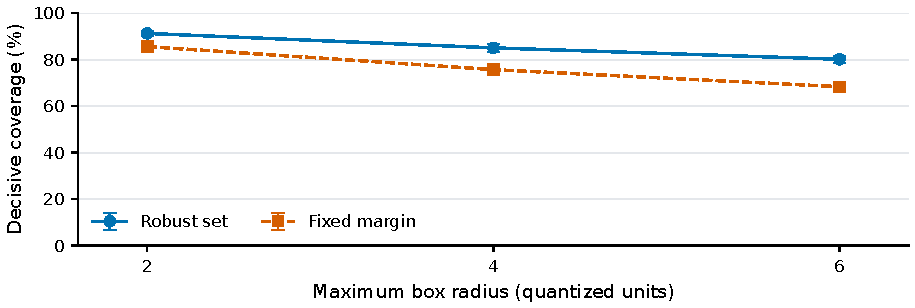
\includegraphics[width=\linewidth]{figures/availability.pdf}
\caption{Decisive coverage for calibrated correlated errors and one Byzantine source. Error bars are normal 95\% intervals over 30 simulation seeds. The horizontal scale is quantized units, with no physical-unit calibration in this synthetic experiment.}\label{fig:availability}
\end{figure}

\subsection{Stress tests outside the security assumptions}
Table~\ref{tab:assumption-stress} violates one premise at a time. Undercoverage yields wrong decisive outputs without inconsistency, while two actual Byzantine sources under a budget of one produce much larger error and evidence-failure rates. Thus ``inconsistent'' is not a general assumption-violation detector.

\begin{table}[htbp]
\centering\small
\caption{Focus-condition stress tests outside the stated source assumptions. Rates are mean seed-level percentages.}
\label{tab:assumption-stress}
\begin{tabularx}{\linewidth}{@{}>{\raggedright\arraybackslash}Xrrrr@{}}
\toprule
Condition & FA & FR & Evidence failure & Decisive\\
\midrule
Undercovered evidence; Byzantine count within budget & 0.23 & 3.41 & 0 & 84.92\\
Two Byzantine sources; verifier budget $f=1$ & 11.62 & 60.86 & 83.33 & 16.67\\
\bottomrule
\end{tabularx}
\end{table}

On the UrbanNav path, nominal simulated evidence gives 93.27\% robust decisive coverage versus 81.94\% for fixed margin, with no observed error for either; the median point has 0.29\% false acceptance and 3.12\% false rejection. Fourfold common bias raises robust rates to 0.032\% and 0.493\%. These are simulated-evidence results, not calibration validation.

\subsection{Effect of the honest-miscoverage budget}
Varying $r$ in Table~\ref{tab:miscoverage} lowers decisive coverage from 85.04\% to 77.46\% under calibrated evidence, with no observed errors. Undercoverage reduces false rejection from 3.41\% to 0.94\% but also reduces decisive coverage from 84.92\% to 78.50\%. Lower $k=n-f-r$ expands the feasible set and makes universal acceptance more conservative; it does not improve evidence calibration.
\begin{table}[htbp]
\centering\small
\caption{Matched miscoverage-budget ablation. Mean seed-level percentages; $n=5,f=1$, radius four, one Byzantine source.}\label{tab:miscoverage}
\begin{tabular}{lrrrr}
\toprule Error model&$r$&False accept&False reject&Decisive coverage\\\midrule
Calibrated&0&0&0&85.04\\
Calibrated&1&0&0&81.25\\
Calibrated&2&0&0&77.46\\
Undercovered&0&0.23&3.41&84.92\\
Undercovered&1&0&1.79&81.67\\
Undercovered&2&0&0.94&78.50\\\bottomrule
\end{tabular}
\end{table}

Figure~\ref{fig:budget} visualizes the matched availability--error tradeoff; negative lower error-bar endpoints are normal-approximation artifacts.
\begin{figure}[htbp]
\centering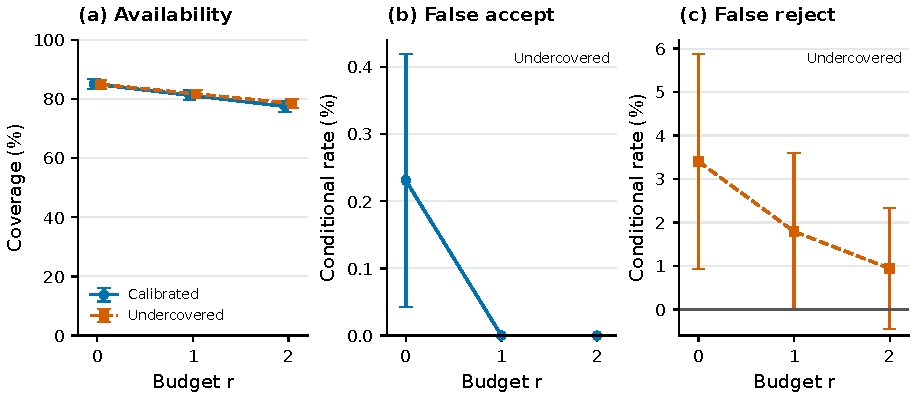
\includegraphics[width=\linewidth]{figures/budget_tradeoff.pdf}
\caption{Honest-miscoverage sensitivity at $n=5,f=1$. Points are seed means; bars are normal 95\% intervals over the same 30 seeds. Calibrated FA/FR are zero for all budgets.}\label{fig:budget}
\end{figure}

\subsection{Hidden-point ZK lower bound}
Table~\ref{tab:point-zk} gives a deliberately weaker same-stack hidden-point lower bound with no signatures, uncertainty, threshold fusion, Byzantine budget, or four-valued output.

\begin{table}[htbp]
\centering\small
\caption{Private point-in-policy Groth16 lower bound. No issuer authentication or robust evidence semantics are included.}
\label{tab:point-zk}
\begin{tabular}{rrrr}
\toprule Dimension & Constraints & Proof bytes & Public witness bytes\\
\midrule
2 & 408 & 164 & 268\\
3 & 612 & 164 & 396\\
\bottomrule
\end{tabular}
\end{table}

The smallest subset circuits use 32,474 constraints at $(3,2)$ and 35,248 at $(3,3)$, versus 408 and 612 for the point predicate. The difference includes signatures, roster/range checks, uncertainty fusion, and four-valued geometry; it is not attributable to robustness alone. Groth16 proof size remains 164 bytes.


\subsection{Quantitative context against recent related systems}
Table~\ref{tab:recent-context} gives source-reported 2024--2026 context without ranking heterogeneous systems. Table~\ref{tab:zklp-repro} then reproduces the closest open Groth16/BN254 location implementation, ZKLP~\cite{ZKLP}, on the same runner.

\begin{table}[htbp]
\centering\footnotesize
\caption{Quantitative context from recent related systems. Values are source-reported and are not normalized into a performance ranking because the certified objects, hardware, and protocols differ.}
\label{tab:recent-context}
\begin{tabularx}{\linewidth}{@{}>{\raggedright\arraybackslash}p{0.16\linewidth}>{\raggedright\arraybackslash}p{0.31\linewidth}>{\raggedright\arraybackslash}X@{}}
\toprule
Work & Evaluation scale & Source-reported result and comparison boundary\\
\midrule
BFT-PoLoc~\cite{BFTPoLoc} (2024) & Up to 450 challengers & At 450 challengers, $\sim$45\% below 100~km and $\sim$95\% below 1000~km uncertainty; Byzantine geolocation, no ZK.\\
PG~\cite{PG} (2024) & 261 cloud / 19 constrained sensors & Private Byzantine sensor fusion with guaranteed delivery; distributed GC protocol.\\
ZKLP~\cite{ZKLP} (2025) & Floating-point location SNARK & Proximity proof $\sim$0.26~s; $\sim$470 peers/s verification; hidden-point geometry.\\
Vehicle ZK-PoL~\cite{VehiclePolicy} (2025) & Up to 43,800 trajectory points & $\sim$36~min EV-subsidy and $\sim$59~min highway proof; trajectory-wide interactive setting.\\
CRSF~\cite{CRSF} (2026) & Up to 261 sensors & Reported online phases $\sim$0.8--1.55~s; collusion-resilient GC fusion, not policy certification.\\
\bottomrule
\end{tabularx}
\end{table}

We pin ZKLP to commit \texttt{e8e3215...62c4} and run its first ZKLP32 vector on the same GitHub Actions Ubuntu runner as a fresh $(n,d)=(3,2)$ subset benchmark. Both use Groth16/BN254 and ten proofs after setup; ZKLP uses a gnark v0.9.1-based fork and ours v0.14.0. The comparison is therefore descriptive, not library- or security-equivalent.

\begin{table}[htbp]
\centering\small
\caption{Same-runner reproduction against the pinned ZKLP implementation. Median times are over ten proofs after one setup. The relations and gnark versions differ, so the table is descriptive rather than a speed ranking.}
\label{tab:zklp-repro}
\begin{tabularx}{\linewidth}{@{}>{\raggedright\arraybackslash}p{0.24\linewidth}rrrrr@{}}
\toprule
Implementation & Constraints & Prove p50 & Verify p50 & Proof bytes & Public bytes\\
\midrule
ZKLP32 pinned smoke & 19,467 & 515.53 & 1.739 & 196 & 140\\
This work, subset $(3,2)$ & 32,474 & 645.14 & 1.547 & 164 & 556\\
\bottomrule
\end{tabularx}
\end{table}

ZKLP certifies hidden point geometry; our row additionally verifies three signed uncertainty boxes, roster/context binding, threshold support, and the robust decision, explaining the larger public witness and circuit. ZKLP's repository also contains an older m6i.xlarge artifact with 21,878 constraints and 270.03~ms median proving time, while the pinned code compiles to 19,467 constraints here. We treat this as version/environment drift, not a performance trend.


\subsection{Real proof costs}
Table~\ref{tab:crypto} reports proof costs. Proofs are 164 bytes for every tested shape; public witnesses are 556--748 bytes, excluding report payload and transport.

\begin{table}[htbp]
\centering\small
\caption{Measured lower-corner Groth16 costs. Times are milliseconds except setup (seconds). Each row uses 30 proofs after one setup.}\label{tab:crypto}
\begin{tabular}{rrrrrrr}
\toprule $(n,d)$&Constraints&Setup&Prove p50&Prove p95&Verify p50&Verify p95\\\midrule
$(3,2)$&55,987&3.64&213.12&244.83&1.033&1.350\\
$(4,2)$&97,493&7.47&360.74&427.17&1.081&1.514\\
$(5,2)$&158,781&11.56&574.69&700.49&1.073&1.212\\
$(3,3)$&185,229&13.84&548.33&707.35&1.067&1.412\\
$(4,3)$&510,362&38.34&1090.95&1212.54&1.093&1.506\\\bottomrule
\end{tabular}
\end{table}

\begin{figure}[htbp]
\centering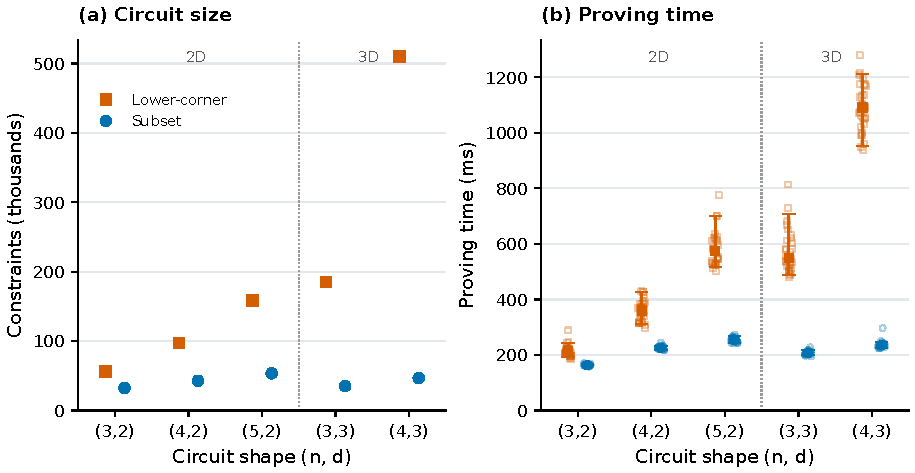
\includegraphics[width=\linewidth]{figures/backend_costs.pdf}
\caption{Matched circuit sizes and measured proving costs for both backends on the Apple M1 workstation. Right: small filled markers show all 30 timings per shape and backend (300 in total); larger markers denote medians and bars span sample p5--p95, not confidence intervals. Horizontal offsets separate observations without changing their values. Backend batches were not interleaved.}\label{fig:scaling}
\end{figure}
For $(n,d)=(4,3)$, the depth backend uses 510,362 constraints and 1.09~s median proving time, versus 46,737 constraints and 234.93~ms for subset enumeration. Subset is smaller in every tested $k=n-1$ case. Batches were measured separately, so timing ratios are descriptive; deployment also requires a trusted setup.

\begin{table}[htbp]
\centering\small
\caption{Matched subset-backend measurements, $k=n-1$, 30 proofs per row. Median times are milliseconds.}\label{tab:subset}
\begin{tabular}{rrrr}
\toprule $(n,d)$&Constraints&Prove p50&Verify p50\\\midrule
$(3,2)$&32,474&163.42&1.028\\
$(4,2)$&42,918&225.79&1.038\\
$(5,2)$&53,528&254.66&1.051\\
$(3,3)$&35,248&206.34&1.059\\
$(4,3)$&46,737&234.93&1.038\\\bottomrule
\end{tabular}
\end{table}

\subsection{Circuit growth and resource boundaries}
Of 32 compilation cases, 27 complete and five hit the sampled RSS limit. At $n=16,d=2$, depth uses 3,509,645 constraints versus 181,194 for subset $k=15$ and 308,978 for $k=14$; balanced subsets grow faster (962,018 at $n=12,d=3,k=6$). Resource-limited counts remain unobserved, and completed overlapping cases show no constraint-count crossover.
\begin{figure}[htbp]
\centering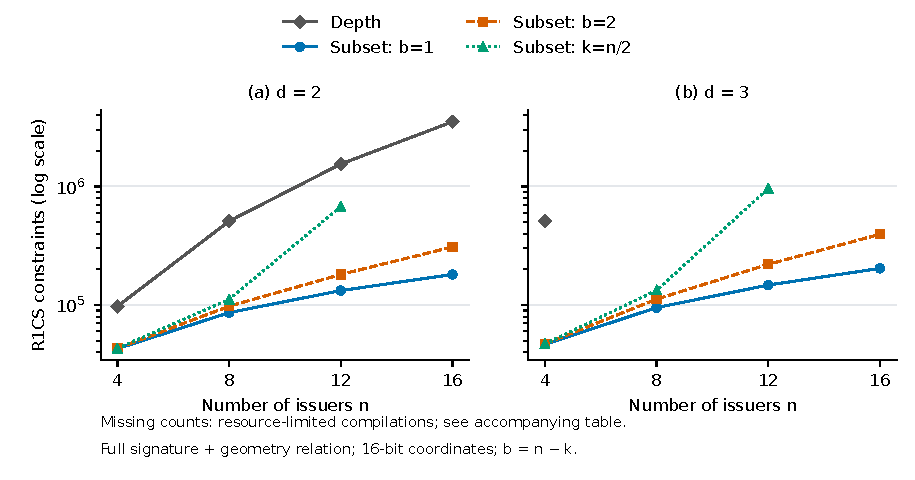
\includegraphics[width=\linewidth]{figures/compile_scalability.pdf}
\caption{Complete-circuit constraint counts. Missing points are resource-limited runs, not zeros; lines only guide the eye. The sweep measures compilation, not proving latency.}\label{fig:compilegrowth}
\end{figure}
\begin{table}[htbp]
\centering\small
\caption{Full R1CS counts. RL: process terminated after sampled RSS exceeded 3~GiB; the constraint count is unobserved.}\label{tab:compilegrowth}
\begin{tabular}{rrrrrr}
\toprule $d$&$n$&Depth&Subset $b=1$&Subset $b=2$&Subset $k=n/2$\\\midrule
2&4&97,493&42,918&43,160&43,160\\
2&8&509,277&86,354&97,734&111,776\\
2&12&1,544,390&132,447&181,221&675,759\\
2&16&3,509,645&181,194&308,978&RL\\
3&4&510,362&46,737&47,099&47,099\\
3&8&RL&95,153&112,213&133,255\\
3&12&RL&147,506&220,640&962,018\\
3&16&RL&203,793&395,417&RL\\\bottomrule
\end{tabular}
\end{table}

\section{Limitations and deployment implications}
The proof certifies a relation between authenticated uncertainty boxes and a public policy; it does not establish physical calibration, independence of nominal issuers, or truth of the report payload. Synthetic experiments control source coverage, and the UrbanNav study uses simulated evidence on a measured path. Appendix~\ref{app:receiver} further shows poor transfer of one retrospective calibration rule. Real deployment therefore requires held-out calibration for each source/regime and governance for common-mode failures.

The fixed roster prevents selective evidence omission but allows one withholding issuer to abort. Distinct keys and trust-domain labels do not prove independent control. Durable replay state, distributed atomicity, revocation, anonymous networking, duplicate-report suppression, and rate limiting remain system-layer requirements.

Zero knowledge hides the witness, not the public classification, roster, policy, threshold, or context; repeated adaptive policies can leak additional location information. Performance measurements are workstation proof-kernel results, not OBU energy or end-to-end V2I latency. Groth16 also requires trusted setup. These limits bound deployment claims but do not change the finite relation proved by the circuit.
\section{Conclusion}
We presented a privacy-preserving certificate for spacetime compliance when evidence is uncertain and some authenticated sources may be Byzantine. Acceptance requires every threshold-supported state to satisfy the task policy, while invalid, ambiguous, and inconsistent evidence remain distinct.

Two Groth16 realizations, a report-bound gateway, adversarial tests, semantic stress tests, same-stack lower bounds, and a pinned ZKLP reproduction validate the finite security relation and its cost. Subset enumeration is substantially cheaper in the tested small-omission regime. The remaining empirical gap is physical multisource calibration: the present result supplies the protocol and reproducible implementation, not a claim of field-ready positioning.
\section*{Funding}
% Funding statement supplied by the user on 2026-09-22; letter O in D2O25O185 retained.
\begingroup\raggedright
This work was supported in part by the Heilongjiang Provincial University Teacher Scientific Research Business Fee under Grant 2018-KYYWF0941, in part by the Heilongjiang Provincial Natural Science Foundation Joint Fund Cultivation Project under Grant PL2024F002, in part by the National Foreign Expert Key Support Project under Grant D2O25O185, and in part by the Heilongjiang Provincial Undergraduate University Excellent Young Teacher Fundamental Research Support Plan under Grant YQJH2024239.

\par\endgroup
\section*{Author contributions}
Lili He: Supervision. Sheng Jiang: Methodology, Software, Investigation. Linghui Lyu: Writing -- original draft. Lei Zhang: Supervision.

\section*{Data and code availability}
The source code, synthetic evaluation scripts, raw benchmark measurements, processed experimental artifacts, and trajectory-replay records supporting this study are available in the public project repository at \url{https://github.com/js110/Apaper}. Third-party datasets used in the study, including UrbanNav and GraphGNSSLib data, remain available from their original sources cited in this article and are not redistributed by the authors.

\appendix
\setcounter{table}{0}
\renewcommand{\theHtable}{appendix.\arabic{table}}
\section{Retrospective single-receiver calibration diagnostic}\label{app:receiver}
GraphGNSSLib's TST2 data~\cite{GraphGNSSData} provide 157 matched static-reference epochs from precomputed RTKLIB 2.4.2 kinematic combined solutions. Horizontal residuals are projected east--north at the repository reference without fitted alignment, bias correction, filtering, or interpolation; vertical residuals are excluded because height/antenna conventions are unverified.

We pre-specified 78 calibration epochs, a ten-epoch gap, and 69 evaluation epochs. With $s_j=\max(|e_j|,|n_j|)$, the 76th ordered calibration score gives a 0.863506~m square half-width. We also evaluate the solution file's reported east/north $3\sigma$ rectangle.

\begin{table}[htbp]
\centering\small
\caption{Reference containment in the static receiver diagnostic. Counts are contained epochs / available epochs; epochs are not independent trials.}\label{tab:receiver}
\begin{tabular}{lrr}
\toprule Rule&Calibration segment&Evaluation segment\\\midrule
Reported $3\sigma$ rectangle&8/78&0/69\\
Calibrated square (0.863506~m)&76/78&2/69\\\bottomrule
\end{tabular}
\end{table}

The calibrated square contains 76/78 calibration references but only 2/69 evaluation references; the reported $3\sigma$ rectangle contains 8/78 and 0/69. Median horizontal residual rises from 0.869 to 1.038~m, with a 1.522~m evaluation maximum. Because the sequence is serially dependent and uses combined processing, this retrospective split supplies neither iid coverage intervals nor online validation. It is a failure diagnostic for one calibration prescription, not a multisource or signed-evidence experiment.

\begin{figure}[htbp]
\centering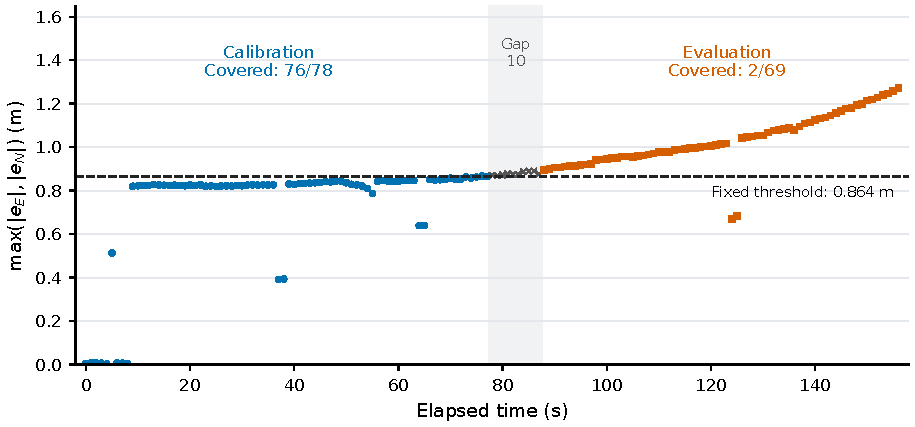
\includegraphics[width=\linewidth]{figures/receiver_diagnostic.pdf}
\caption{Static-receiver diagnostic. All 157 matched epochs are shown; the dashed line is the fixed 0.863506~m square half-width. Combined processing and serial dependence prevent an online-coverage interpretation.}\label{fig:receiver}
\end{figure}
\section*{Declaration of generative AI and AI-assisted technologies in the manuscript preparation process}
During the preparation of this work, the authors used OpenAI ChatGPT and OpenAI Codex to assist with language editing, manuscript organization, revision of presentation, code-level editing and checking, and preparation of explanatory schematics. Model-version identifiers were not exposed in the retained workflow records. After using these tools, the authors reviewed and edited the content as needed and take full responsibility for the content of the publication.

% If generative AI was used to create or modify any submitted figure, add the corresponding tool disclosure to that figure caption before submission, as required by Elsevier policy.
\bibliographystyle{elsarticle-num}
\bibliography{references}
\end{document}
